% \cleardoublepage
\chapter{Approach and Design}\label{sec:approach_design}\minitoc\vspace{.5cm}
\index{Approach and Design}

By employing AF_XDP sockets for the Receiver-Transmitter layer (RX-TX), we can achieve multipath tunneling that offers exceptional performance and grants complete control over raw IP packets before they enter the Linux network stack. 
Thanks to the secure design of the eBPF virtual machine architecture, this approach remains safer compared to utilizing kernel modules or kernel code used by Wireguard, OpenVPN, and IPsec, ...
In this chapter, we will explore the concept and design of the tunnel by examining its intended features and components.

\section{Multipath Tunnel using XDP socket}
- A modern approach to system and network programming: performance, safe and free from legacy code thanks to eBPF-AF_XDP technology.
- Almost certainly will heavily outperform any other user-space approach
- Increase redundancy and connection reliability.
- Possible improvement in latency
- Disparity in line utilization to support different types of streams: data need bandwidth, voice-over-ip needs low latency, critical message needs reliable transmission

- The MTX tunnel allows setting policies at several layers defined by algorithms or configuration. With such preemptive points these will be a large pool of configurations to chose from:
	- Data link layer: which stream can use which link, with which priority, what is the load distribution policy?
	- Network layer: select IPv4/v6 as carrier, which UDP port.
	- Application layer: priority of application, buffer fetching timeout, buffer reserved for low-latency usage, ...
- Ideally, after initiation, a tunnel control plane will run in background and manage the streams that are used by several applications. These applications register usage to the tunnel control plane and interact with data plane through shared buffers. Parameters can be set individually for each app.
- Apart from that, we will also investigate the possibility to create a TUN/TAP interface as a intermediate communicate layer between the MTX tunnel and apps. This is a well-known practice used by many VPN programs to allow several apps to use the VPN connection. This way, applications can use the tunnel connection without modifying the source code.

\section{AF\_XDP socket - eBPF}
High throughput: kernel-bypass method such as DPDK and AF_XDP can easily saturate 100Gbit line per core on a modern CPU, with baseline packet drop per second of up to 43.5Mpps (million packets per second) and 24Mpps respectively compared to 4.8Mpps by Linux networking stack \CITE{hoiland_jorgensen_express_2018} \cite{intel_dpdk_perf}.
his provides us the opportunity to create a multi-hundreds Gbit connection (tunnel) using nothing more than just several available 40/100Gbit NIC.


\section{Implementation details}
% \section{Introduction}

% \begin{wrapfigure}{r}{0.2\textwidth}
%     \centering
%     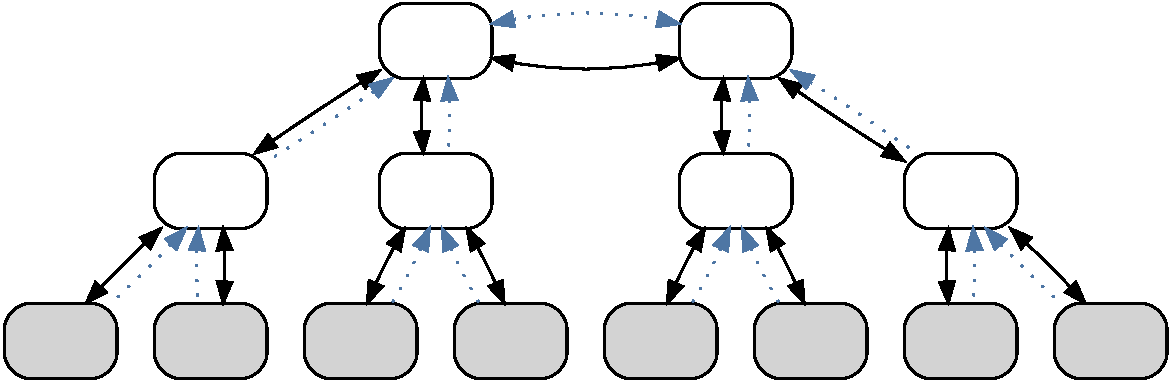
\includegraphics[width=0.2\textwidth]{resources/images/example3}
% \end{wrapfigure}

% \sidenote{Overview}
% \todomid{write about \Cref{fig:req:details}}

% \begin{figure}[H]
%     \centering
%     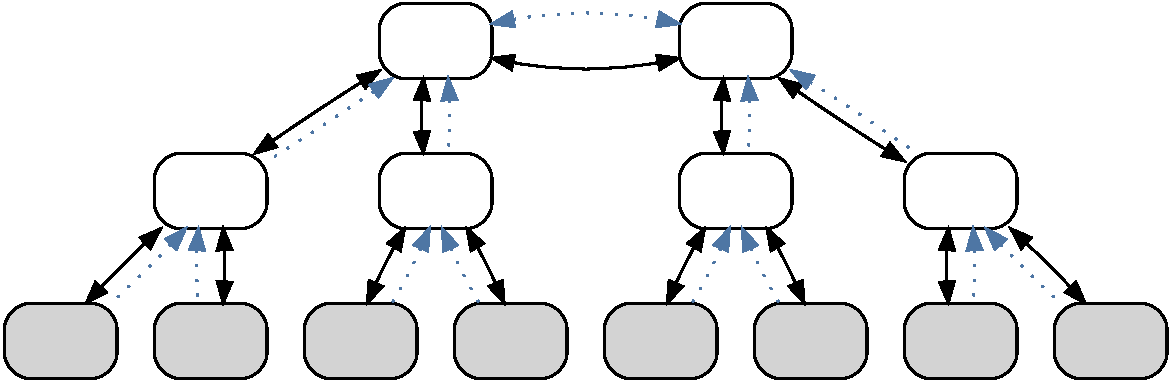
\includegraphics[width=.85\textwidth]{resources/images/example3}
%     \caption{More detailed overview of the requirements}\label{fig:req:details}
% \end{figure}

% \sidenote{Structure of Research}
% \todomid{write about \Cref{fig:hourglass:reqs}}

% \begin{figure}[H]
%     \centering
%     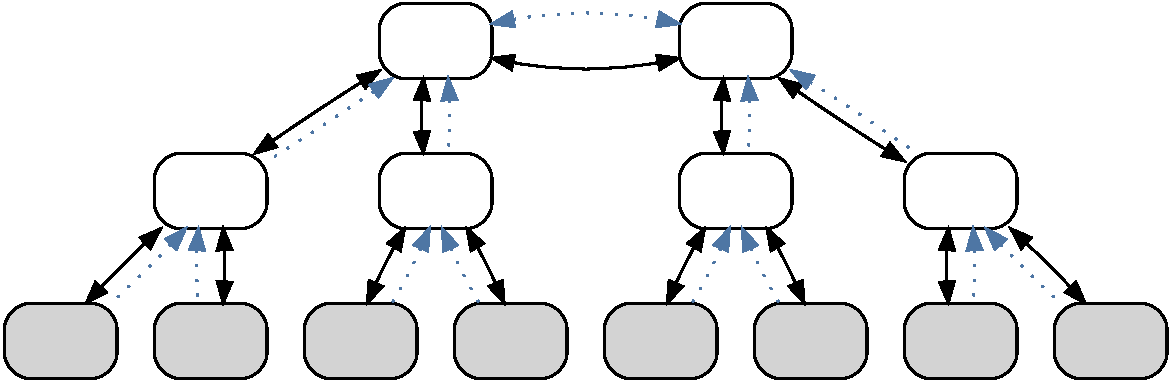
\includegraphics[width=.55\textwidth]{resources/images/example3}
%     \caption{Placement of the requirement section in the structure of research}\label{fig:hourglass:reqs}
% \end{figure}

% \section{Stakeholder 1}

% \sidenote{\Cref{tbl:reqs:stakeholder1}}
% \todomid{write about \Cref{tbl:reqs:stakeholder1}}

% \begin{tabularx}{\textwidth}{lX}
%     \caption{Requirements from stakeholder 1 perspective}\label{tbl:reqs:stakeholder1}\\
%     \toprule
%     \textbf{\#}& \textbf{Description}  \\\midrule
%     \endfirsthead%
%     \toprule
%     \textbf{\#}& \textbf{Description}  \\\midrule
%     \endhead%
%     \requirement{U}{req:stakeholder1:foo}{Foo}
%        & \todomid{write}
%     \\\midrule
%     \requirement{U}{req:stakeholder1:bar}{Bar}
%        & \todomid{write}
%     \\\bottomrule
% \end{tabularx}

% \section{Stakeholder 2}

% \sidenote{\Cref{tbl:reqs:stakeholder2}}
% \todomid{write about \Cref{tbl:reqs:stakeholder2}}

% \begin{tabularx}{\textwidth}{lX}
%     \caption{Requirements from stakeholder 2 perspective}\label{tbl:reqs:stakeholder2}\\
%     \toprule
%     \textbf{\#}& \textbf{Description}  \\\midrule
%     \endfirsthead%
%     \toprule
%     \textbf{\#}& \textbf{Description}  \\\midrule
%     \endhead%
%     \requirement{S}{req:stakeholder2:foo}{Foo}
%        & \todomid{write}
%     \\\midrule
%     \requirement{S}{req:stakeholder2:bar}{Bar}
%        & \todomid{write}
%     \\\bottomrule
% \end{tabularx}

% \section{Stakeholder 3}

% \sidenote{\Cref{tbl:reqs:stakeholder3}}
% \todomid{write about \Cref{tbl:reqs:stakeholder3}}

% \begin{tabularx}{\textwidth}{lX}
%     \caption{Requirements from stakeholder 3 perspective}\label{tbl:reqs:stakeholder3}\\
%     \toprule
%     \textbf{\#}& \textbf{Description}  \\\midrule
%     \endfirsthead%
%     \toprule
%     \textbf{\#}& \textbf{Description}  \\\midrule
%     \endhead%
%     \requirement{T}{req:stakeholder3:foo}{Foo}
%        & \todomid{write}
%     \\\midrule
%     \requirement{T}{req:stakeholder3:bar}{Bar}
%        & \todomid{write}
%     \\\bottomrule
% \end{tabularx}

% \section{Conclusion}

% \sidenote{Summary}
% \todomid{write}

% \sidenote{Takeaway 1}
% \todomid{write}

% \sidenote{Takeaway 2}
% \todomid{write}

% \sidenote{Takeaway 3}
% \todomid{write}

% \sidenote{Next chapter}
% \todomid{write}
